\documentclass{standalone}

\usepackage{tikz}
\usetikzlibrary{arrows}
\usepackage{amsfonts,amssymb,amsmath}

\begin{document}
\pagestyle{empty}
%
\tikzstyle{int}=[draw, fill=blue!20, minimum size=2em]
\tikzstyle{init} = [pin edge={to-,thin,black}]
%
%\begin{tikzpicture}[->,auto,node distance=1.5cm,
%  thick,gauge node/.style={circle,draw},matter node/.style={rectangle,draw}]
%
%  \node[gauge node] (1) {1};
%  \node[gauge node] (2) [right of=1] {2};
%  \node (3) [right of=2] {$\cdots$};
%  \node[gauge node] (4) [ right of=3] {$N$};
%  \node[matter node] (5) [ right of=4, minimum height=0.9cm] {$N+1$};
%  
%   \path[every node/.style={font=\sffamily\small}]
%    (1) edge node [bend left]  {} (2)
%    (2) edge node [right] {} (3)
%    (3) edge node [right] {} (4)
%    (4) edge node [left] {} (5);
%\end{tikzpicture}

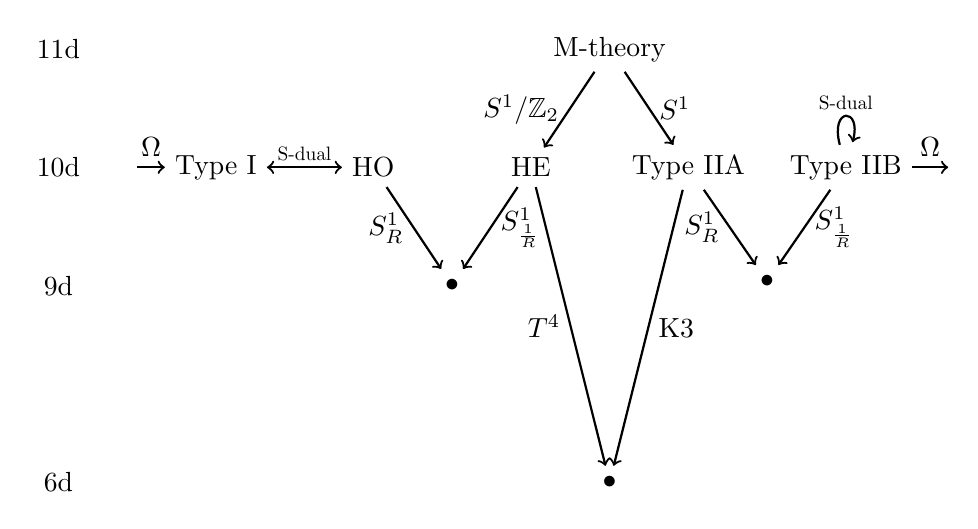
\begin{tikzpicture}[auto,node distance=2cm,
  thick,gauge node/.style={},matter node/.style={rectangle,draw}]


   
  \node[gauge node] (10) {10d};
   \node[gauge node] at (0,1.5) {11d};
      \node[gauge node]  at (0,-1.5) {9d};
      \node[gauge node] at (0,-4) {6d};
  \node[gauge node] (11) [right of=10] {Type I};
  \node[gauge node] (12) [right of=11] {HO};
  \node [gauge node] (13) [right of=12] {HE};
    \node [gauge node] (01) at (7,1.5) {M-theory};
  \node[gauge node] (14) [ right of=13] {Type IIA};
    \node[gauge node] (22) at (9,-1.45) {$\bullet$};
  \node[gauge node] (15) [ right of=14] {Type IIB};
       \node[gauge node] (21) at (5,-1.5) {$\bullet$};
       \node[gauge node] (31) at (7,-4) {$\bullet$};

\begin{scope}
  \draw [->] (1,0) to node [midway] {$\Omega$} (11);
    \draw[->]   (01) to [ left] node [midway] {$S^1/\mathbb{Z}_2$} (13);
    \draw[->]   (01) to [ right] node [midway] {$S^1$} (14);
  \draw [<->] (11) to  node [above,scale=.7]{S-dual} (12);
   \draw[->]   (12) to [ left] node [midway] {$S_R^1$} (21);
      \draw[->]   (13) to [ right] node [midway] {$S_{\frac1R}^1$} (21);
         \draw[->]   (14) to [ left] node [midway] {$S_R^1$} (22);
      \draw[->]   (15) to [ right] node [midway] {$S_{\frac1R}^1$} (22);
               \draw[->]   (13) to [ left] node [midway] {$T^4$} (31);
      \draw[->]   (14) to [ right] node [midway] {K3} (31);
%    \draw (11) to  node [right,scale=.7]{$Q_1$} (22);
%  \draw (21) to  node [right,scale=.7]{$P_1$} (11);
%  \draw [<->] (14) to node [above,scale=.7]{$B_2$} (15);
%    \draw (12) to node [right,scale=.7]{$Q_2$} (23);
%  \draw (22) to  node [right,scale=.7]{$P_2$} (12);
%    \draw (13) to node [above,scale=.7]{$B_{M-1}$} (14);
%        \draw (13) to node [ right,scale=.7]{$Q_{M-1}$} (24);
%       \draw (14) to  node [above,scale=.7]{$B_{M}$} (15);
%  \draw (24) to  node [right,scale=.7]{$P_{M}$} (14);
%    \draw (14) to  node [right,scale=.7]{$Q_{1}$} (25);
% \draw (25) to  node [right,scale=.7]{$P_{1}$} (15);
     \draw[->] (15) to  node [midway]  {$\Omega$} (11.3,0);
%          \draw (15) to  node [midway]  {} (26);
 
  \end{scope}
   \path[]
%    (11) edge [ loop above] node [above,scale=.7]{$A_1$} (11)
%       (12)     edge [loop above] node [above,scale=.7]{$A_2$} (12)
%           (14) edge [loop above] node [above,scale=.7]{$A_M$} (14)
 (15) edge [loop above] node [above,scale=.7]{S-dual} (15);
\end{tikzpicture}



\end{document}